% !TEX root = ../main.tex

\hyphenation{Dha-ra-ni-pra-ga-da Pad-ma-na-bhan}
\section{REVIEW OF RELATED LITERATURE}
\label{sec:related}

% =====================================================================
% 14 Nov 2026: ported from the unified doc (Pre-Proposal Draft >
% CHAPTER 1 tab, Chapter 2 part), with the Nov 14 review fixes:
% R05 Domain column in Table 2.2; R07 summary of how the image methods
% differ; R08 McNemar, Holm, significance level vs alpha, baseline
% absolute values; typos (UTMOSE, missing parenthesis, "tested threshold",
% Zheng "four times the original speech"); 2.5 cross-reference now
% points to the calibration-size section of Chapter 3 by label.
% R09: LTT-for-TTS paragraph added at the end of 2.5; R16: what the
% teacher passes, in 2.3.
% 18 Nov 2026: aligned with the payload-router Chapter 3 (fixed commit
% point, choice of payload, residual, absolute failure rule, variety
% measured); new Section 2.4 on noisy prompts and histogram equalization.
% 18 Nov 2026 (later): Tables 2.1 and 2.2 grouped by category; Table 2.3
% gives the sources of each added component (panel item 9); passages
% tied only to the old stopping-time scheduler removed.
% =====================================================================

\subsection{Flow-Matching Speech Synthesis and Its Computational Cost}
\label{sec:rrl-fm}

\subsubsection{Flow Matching}

A generative model has to turn something easy to sample, such as random Gaussian noise, into something hard to sample, such as the acoustic features of speech. Flow matching does this by learning a \emph{velocity field}: for every point and every time $t$ between 0 (noise) and 1 (data), the field says in which direction the point should move so that noise ends up as data \parencite{lipman2023flow,lipman2024guide,liu2023flow}. Generating a sample then means starting from noise and following the field from $t=0$ to $t=1$, that is, solving an ordinary differential equation (ODE), $\mathrm{d}x/\mathrm{d}t = v_\theta(x,t)$, where $v_\theta$ is the network. The network is trained on the straight path $x_t=(1-t)x_0+t x_1$ between a noise sample $x_0$ and a data sample $x_1$, whose velocity is simply $x_1-x_0$; this makes training simple and needs no simulation of the ODE \parencite{chen2018neuralode,lipman2023flow}. The point at which the teacher hands over to the student is a point on this $t$ axis.

In practice the ODE is solved in a fixed number of steps. The explicit Euler method \parencite{hairer1993} on a time grid $0=t_0<t_1<\dots<t_N=1$ moves the sample $x_{t_i}$ a small distance along the current velocity at each step (used in Chapter~3 in Algorithm~\ref{alg:baseline}):
\begin{equation}
x_{t_{i+1}} = x_{t_i} + (t_{i+1}-t_i)\, v(x_{t_i}, t_i).
\label{eq:rrl-euler}
\end{equation}
Each step costs one evaluation of the network, and the error of each step shrinks with the step size. With very few, large steps the sample drifts away from realistic speech, which is why few-step generation needs the techniques of Section~\ref{sec:rrl-distill}.

Because the training path is straight, one step of length $1-t$ along the current velocity gives an estimate of the final output from any point on the way \parencite{li2025dmospeech2,lipman2024guide} (defined in Chapter~3 as \Cref{eq:endpoint}):
\begin{equation}
\hat{x}_1(t) = x_t + (1-t)\, v(x_t,t).
\label{eq:rrl-endpoint}
\end{equation}
This \emph{endpoint estimate} costs no extra network evaluation once the velocity is known. In the released DMOSpeech~2 code, it is what the teacher passes to the student \parencite[see also Section~\ref{sec:rrl-handover}]{li2025dmospeech2code}, and in this study it is the teacher's payload, the content that the proposed method either passes on or corrects.

Some samplers add fresh noise during sampling; in score-based models, such a stochastic sampler and its noise-free counterpart describe the same distribution of outputs \parencite{song2021sde}. The released DMOSpeech~2 sampler has an optional stochastic term, which this study will switch off so that the teacher gives the same estimate for the same input.

\subsubsection{Zero-Shot Text-to-Speech}

A zero-shot TTS system receives a few seconds of a new speaker's voice (the prompt), the transcript of the prompt and a target text, and must speak the target text in that voice without being retrained for the speaker. Earlier systems used speaker encoders or language models over audio codes; diffusion and flow-matching systems instead treat the task as filling in the missing part of a mel-spectrogram whose first part is the prompt \parencite{anastassiou2024seedtts,eskimez2024e2,le2023voicebox}. Matcha-TTS showed that conditional flow matching gives fast, high-quality TTS \parencite{mehta2024matcha}. F5-TTS, the teacher in this study, used a diffusion transformer and introduced \emph{sway sampling} \parencite{chen2024f5}, which spaces the solver's time steps unevenly by mapping a uniform grid $u\in[0,1]$ to a flow time $t$ with a sway coefficient $s$ (applied in Chapter~3 as \Cref{eq:grid}):
\begin{equation}
t = u + s\,\big(\cos(\tfrac{\pi}{2}u) - 1 + u\big)
\label{eq:rrl-sway}
\end{equation}
With $s=-1$ the map becomes $t=1-\cos(\tfrac{\pi}{2}u)$, and half of the steps fall below $t\approx0.29$ (Figure~\ref{fig:rrl-sway}). F5-TTS and DMOSpeech~2 both argued that these early steps decide the coarse structure of the output, such as prosody and alignment; DMOSpeech~2 describes sway sampling as allocating \enquote{more samples to early time steps where most of the semantic structure is established} \parencites{chen2024f5}[p.~31818]{li2025dmospeech2}. A training-free pruning of the F5-TTS schedule found that some of these steps are redundant, while noting that \enquote{the precision of later steps depends on the precision of the early steps} \parencite[p.~2]{zheng2025epss}. The handover at $t_{\text{switch}}=0.25$ lies in this dense region, so reaching it takes most of the teacher's work. A coarser grid made of every second point reaches the same handover time in half the steps; the proposed method uses this kind of pruning.

\begin{figure}[!htbp]
\centering
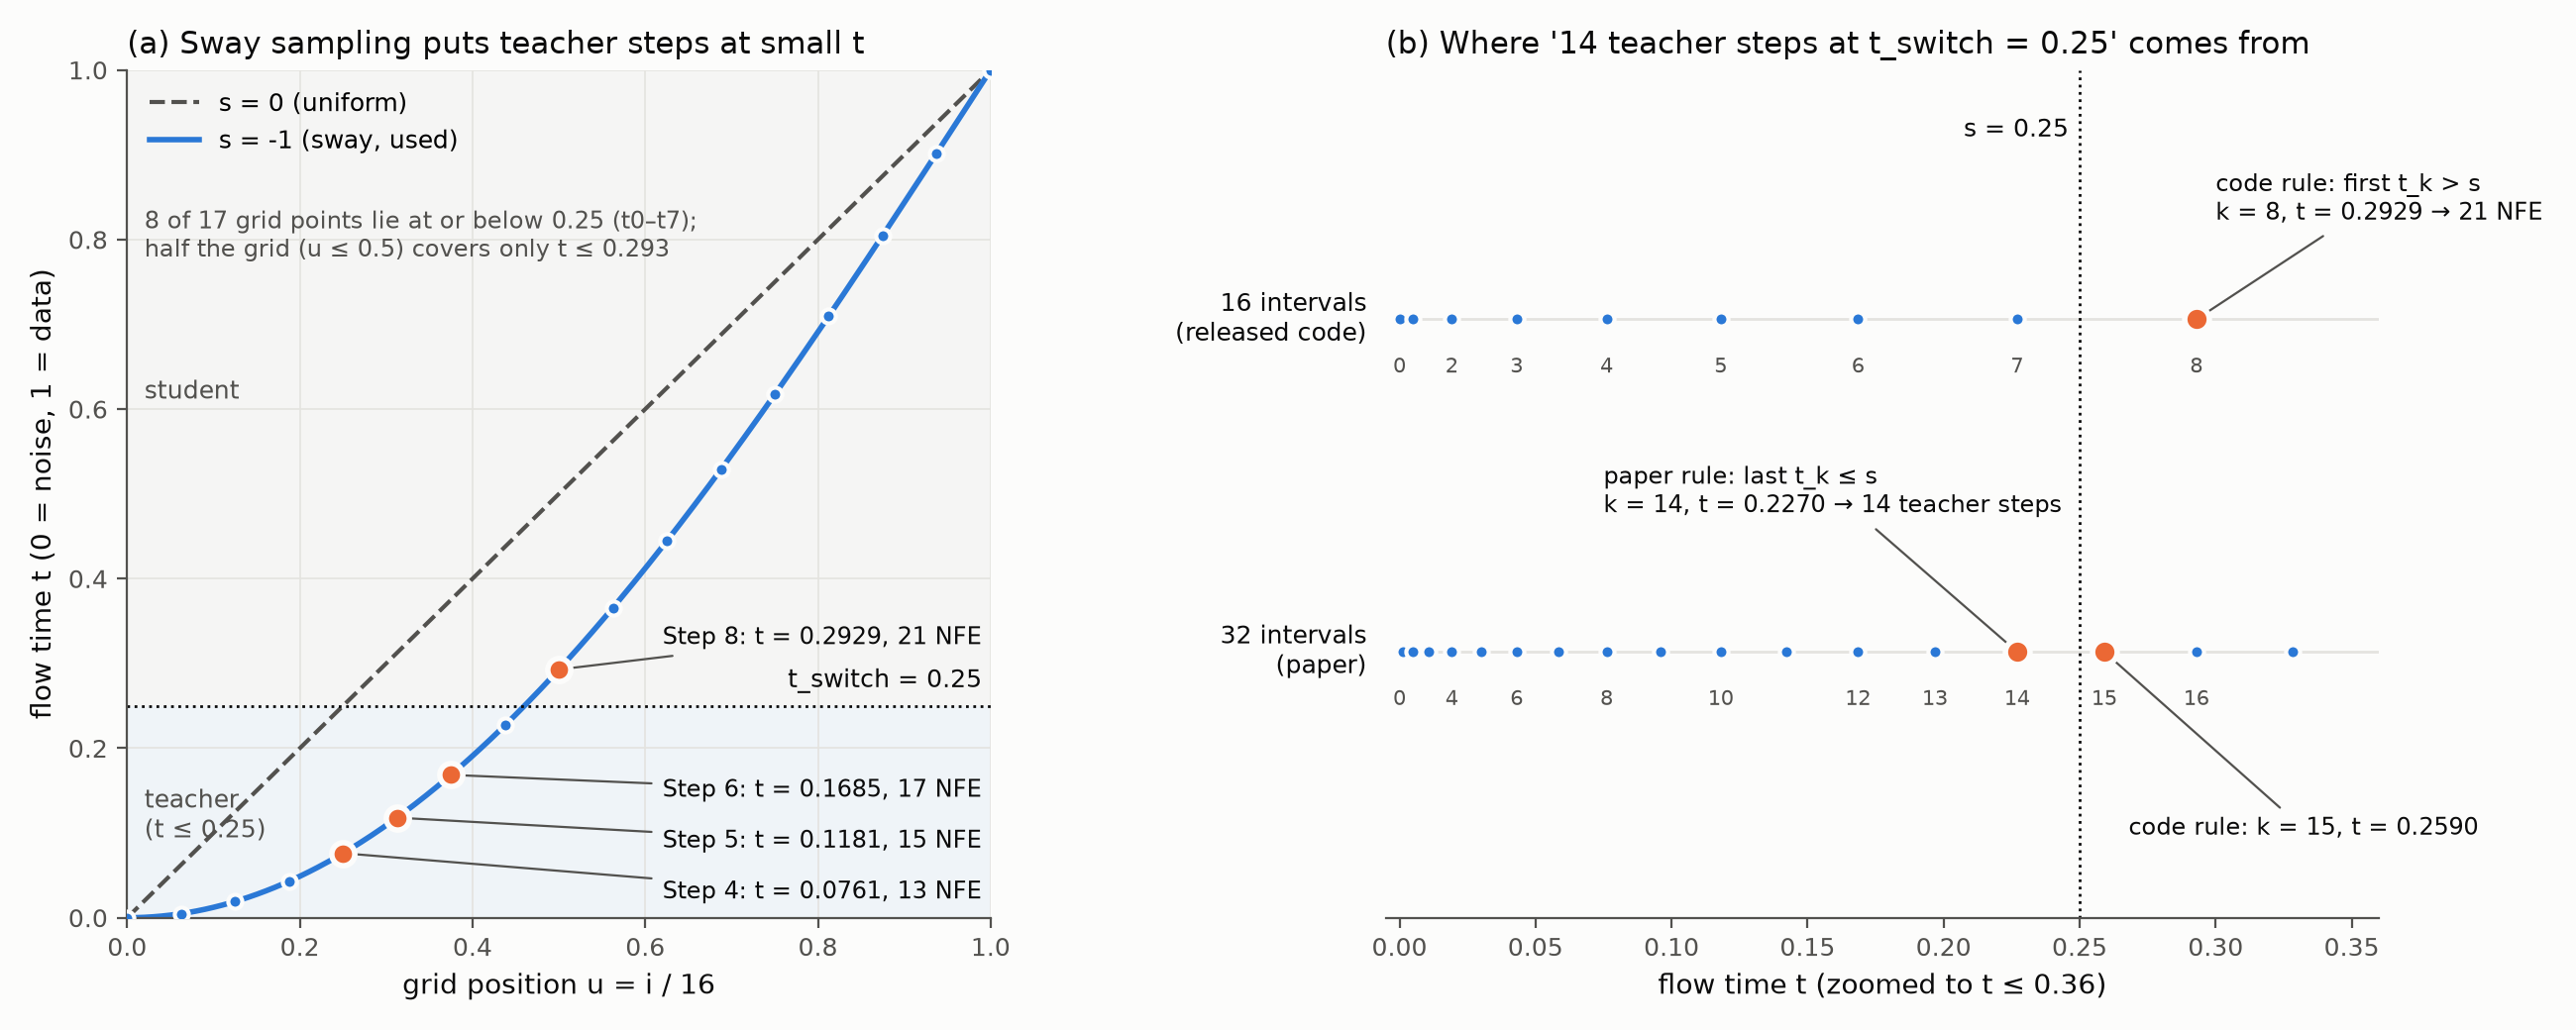
\includegraphics[width=\textwidth]{figures/sway_grid_tswitch.png}
\caption[Sway sampling and the switching time]{Sway sampling ($s=-1$) concentrates teacher steps at small $t$, where the switching time lies. (a) The sway map against the uniform grid; 8 of the 17 teacher grid points lie at or below $t_{\text{switch}}=0.25$, and each additional guided teacher step costs two forward passes, so the released handover after eight steps costs 21 forward passes, and a coarser grid with every second point reaches the same handover time in four steps. (b) Near $t=0.25$, the paper's 14 teacher steps correspond to the last point not above 0.25 on a 32-interval grid ($t_{14}\approx0.227$), while the released code stops at the first point above 0.25 on its 16-interval grid ($t_8\approx0.293$). Figure by the researchers, computed from the sway map of \textcite{chen2024f5}, the configuration reported by \textcite[p.~31819]{li2025dmospeech2} and the released code \parencite{li2025dmospeech2code}.}
\label{fig:rrl-sway}
\end{figure}

\subsubsection{Forward-Pass Cost and Guidance}

Classifier-free guidance (CFG) makes the output follow the text and the speaker prompt more closely by combining two predictions of the same network, one with the condition and one without it, as $v = v_u + w\,(v_c - v_u)$, where $v_c$ and $v_u$ are the conditional and unconditional predictions and $w$ is the guidance weight \parencite{ho2022cfg}. When the two predictions are computed separately, each guided step needs two network evaluations, also called forward passes or neural function evaluations (NFEs). Flow-matching TTS systems count cost the same way: F5-TTS-based models run \enquote{two forward passes at each step} \parencite[p.~2]{yang2025shallow}, and NFEs are counted as \enquote{two for a guided step and one for unguided step} \parencite[p.~2]{lee2026guidance}.

The teacher in DMOSpeech~2 is guided. The student was trained to match the output distribution of the guided teacher, with the guidance built into its training target \parencite[p.~20]{li2024dmospeech}, so it runs without guidance and needs only one pass per step \parencite{li2025dmospeech2}. Counting integration steps alone would therefore understate the cost: the study will count forward passes, and a teacher step costs twice a student step, so the savings lie in the teacher's steps.

% =====================================================================
\subsection{Methods for Reducing Sampling Cost}
\label{sec:rrl-distill}

There are three ways to make sampling cheaper. Better numerical solvers keep the same network and reach a given accuracy in fewer steps \parencite{karras2022edm,lu2022dpmsolver}; every step still costs a full, guided evaluation, so they help less when only a handful of steps are left. Distillation instead trains a \emph{student} network that needs only a few steps. Progressive distillation repeatedly halved the number of steps \parencite{salimans2022progressive}, consistency models learned to map any point on a trajectory directly to its endpoint \parencite{song2023consistency}, and distribution matching distillation (DMD) trained a generator whose outputs follow the teacher's output distribution \parencite{yin2024dmd2,yin2024dmd}. A third route keeps the trained model and changes how it is run, without retraining. For F5-TTS, \textcite{zheng2025epss} inspected the sampling trajectory, identified redundant steps, and proposed \enquote{a training-free, plug-and-play approach} (p.~1) that generates speech in seven steps, about four times faster than the original sampler, while keeping comparable quality. \textcite{sakpiboonchit2025smoothcache} instead reused the outputs of selected transformer layers across sampling steps, which nearly halved the real-time factor of F5-TTS with little loss in quality (p.~6). This study belongs to the third route: it will keep the released Euler sampler and the trained networks, stop the teacher at one fixed, cheaper point, and change only what the teacher hands to the student, so better solvers are complementary and outside its scope.

In speech, DMOSpeech distilled a diffusion TTS teacher with DMD, reduced sampling from 128 steps to four, and added training objectives that directly improve intelligibility and speaker similarity, presenting itself as \enquote{the first distilled TTS model that consistently outperforms its teacher} \parencite[p.~2]{li2024dmospeech}.

The student in this study comes from the DMOSpeech line. It was trained with the improved DMD of \textcite{yin2024dmd2} to match the F5-TTS teacher and generates speech in four steps at the sway-sampled noise levels $t\in\{0,\,0.0761,\,0.2929,\,0.6173\}$ \parencite[p.~31816]{li2025dmospeech2}. Like a consistency model, at each of its few steps it predicts the final output and then mixes that prediction with fresh noise before the next step \parencite[p.~20]{li2024dmospeech}.

Distillation, however, trades diversity for speed. DMOSpeech~2 reported that the distilled student, while similar to the teacher in predicted sound quality, \enquote{demonstrates less diversity in prosodic features such as intonation patterns, rhythm variations, and speech cadences}, a loss it called mode shrinkage \parencite[p.~31818]{li2025dmospeech2}. Because the teacher is kept mainly to restore this diversity, this study will measure it with DMOSpeech~2's pitch-based measure of variety across random seeds (Chapter~3).

% =====================================================================
\subsection{Teacher-Guided Sampling and Re-Noising at the Handover}
\label{sec:rrl-handover}

DMOSpeech~2 restored diversity by letting the teacher perform the first, high-noise steps and the student finish the rest \parencite{li2025dmospeech2}. The point at which the teacher hands its state to the student is the \emph{switching time}; this study fixes it and instead selects what is handed over. What the teacher passes to the student is a single tensor, its estimate of the final mel-spectrogram (\Cref{eq:rrl-endpoint}); no weights, gradients or separate features are transferred, and both models are conditioned on the same text and prompt \parencite{li2025dmospeech2code}. The authors attributed the restored diversity to a division of labour: the teacher's early steps establish \enquote{diverse prosodic patterns and text-speech duration alignments}, and the student's later steps handle \enquote{the refinement of acoustic details} \parencite[p.~31818]{li2025dmospeech2}. Their main configuration used $t_{\text{switch}}=0.25$, with the teacher handling 14 steps and the student 2 \parencite[p.~31819]{li2025dmospeech2}, and they reported outputs about $1.8\times$ faster than the full teacher, which uses 32 steps \parencite[pp.~31818--31819]{li2025dmospeech2}. They suggested a switching time of about 0.1--0.2 when efficiency matters and 0.4--0.5 when diversity matters \parencite[p.~31818]{li2025dmospeech2}. The switching time was a single value for all inputs, so the speed--diversity trade-off was set once rather than per utterance.

Because a guided step costs two forward passes \parencite{ho2022cfg,yang2025shallow} and a student step one \parencite{li2025dmospeech2,li2024dmospeech}, teacher-guided sampling with $K$ guided teacher steps and $M$ unguided student steps, against a full teacher of $N$ steps, costs (the exact count for the released code is \Cref{eq:cost} in Chapter~3)
\begin{equation}
C(K,M) = 2K + M, \qquad \text{speed-up over the full teacher} \approx \frac{2N}{2K+M}
\label{eq:tgcost}
\end{equation}
For the paper's configuration, $K=14$ and $M=2$ give 30 passes against 64 for the full teacher, a ratio of about 2.1. The reported runtime speed-up of about $1.8\times$ is smaller because the duration predictor, the vocoder and data movement do not shrink with the number of forward passes. Because $K$ can only take the values of the teacher grid, the cost changes in steps of two passes as the switching time crosses grid points (Figure~\ref{fig:rrl-tg}). The released DMOSpeech~2 code differs from the paper's description in one important detail: it stops the teacher at the first grid point \emph{above} $t_{\text{switch}}$ on a 16-interval grid, so $t_{\text{switch}}=0.25$ gives eight teacher steps instead of fourteen \parencite{li2025dmospeech2code}. Chapter~3 uses the released code and its exact cost.

Inputs differ in how much of the teacher's work can be trusted. For a clean prompt, the teacher's estimate carries useful prosody; for a noisy prompt, a guided teacher can copy the prompt's noise into its estimate, which the student then inherits (Section~\ref{sec:rrl-noise}). DMOSpeech~2 reported only average results over its test set \parencite[p.~31819]{li2025dmospeech2}, which cannot show such differences. The researchers' preliminary experiments (Appendices~\ref{app:prelim} and~\ref{app:snr-r}) found that early handovers failed mostly on noisy prompts, and that the failures came from noise copied by the teacher rather than from too few teacher steps.

How the student takes over differs between the paper and the released code. In the paper, the student \enquote{completes the remaining denoising process from $t_{\text{switch}}$ to 1} starting from the teacher's state \parencite[p.~31818]{li2025dmospeech2}. In the released code, the student does not continue exactly from the teacher's state. It first \emph{re-noises} the teacher's endpoint estimate $\tilde x$, mixing it with fresh noise $\varepsilon$ at a restart level $\tau$ \parencite{li2025dmospeech2,meng2022sdedit} (used in Chapter~3 in Algorithm~\ref{alg:baseline}):
\begin{equation}
x_\tau = (1-\tau)\,\varepsilon + \tau\,\tilde{x}, \qquad \varepsilon\sim\mathcal{N}(0,I),\; \tau\in[0,1]
\label{eq:rrl-renoise}
\end{equation}
A fraction $\tau$ of the input carries the teacher's information and $1-\tau$ is fresh noise. This is the same operation as SDEdit, which showed that the noise level trades faithfulness to the guide against realism of the output, and that moderate noise keeps the guide's overall layout \parencite{meng2022sdedit}. Restart sampling gave a second reason why re-noising helps: adding noise and solving again shrinks errors accumulated earlier in sampling \parencite{xu2023restart}. Together these explain why the student tolerates an imperfect teacher estimate.

\begin{figure}[!htbp]
\centering
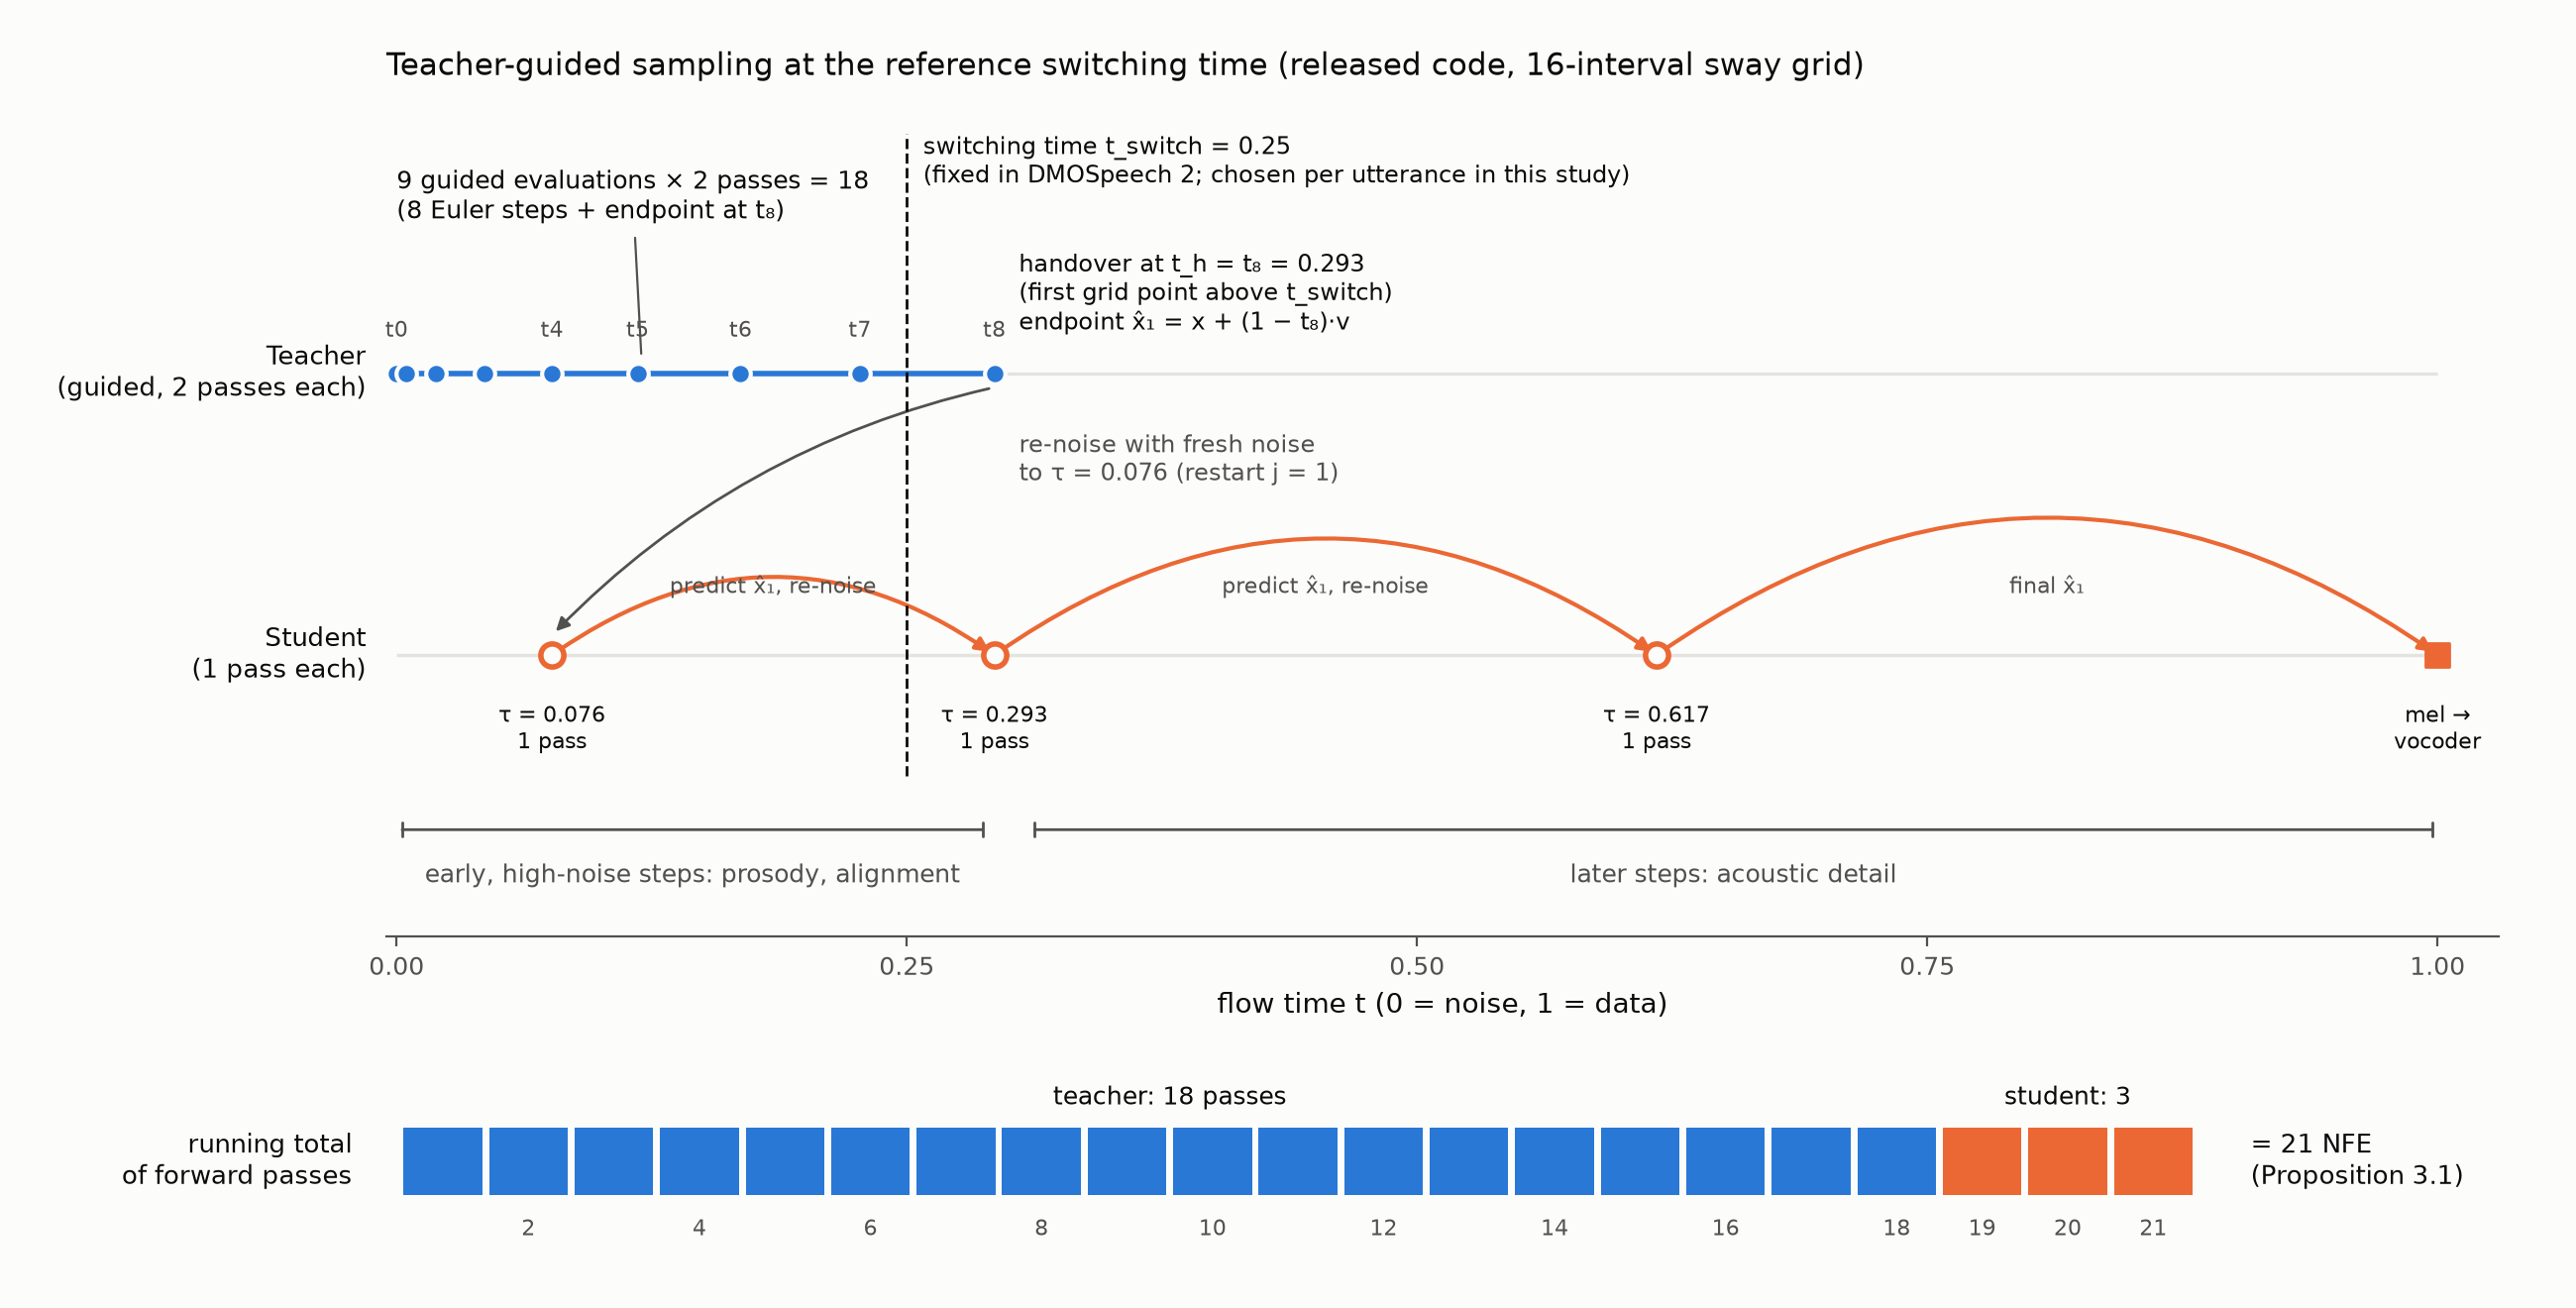
\includegraphics[width=\textwidth]{figures/teacher_guided_timeline_t55.png}
\caption[Teacher-guided sampling in DMOSpeech~2]{Teacher-guided sampling in the DMOSpeech~2 code at the reference switching time ($t_{\text{switch}}=0.25$, 16-interval sway grid). The teacher takes guided Euler steps up to the first grid point above $t_{\text{switch}}$ ($t_8\approx0.293$), and one more guided evaluation gives the endpoint estimate $\hat x_1$. The student then restarts from a re-noised copy of $\hat x_1$ at $\tau\approx0.076$ and finishes in three unguided steps. Guided teacher evaluations cost two forward passes each, so the teacher accounts for 18 of the 21 passes. In DMOSpeech~2 both the switching time and the handed-over content are fixed; this study keeps a fixed, cheaper handover point and chooses per utterance what is handed over. Figure by the researchers, based on the sampler described by \textcite{li2025dmospeech2} and the released code \parencite{li2025dmospeech2code}.}
\label{fig:rrl-tg}
\end{figure}

In the released code the restart level is set by the student's own grid, not by the switching time \parencite{li2025dmospeech2code}. With the default start index the student always restarts at $\tau=0.0761$, which equals the teacher's fourth grid point. For a handover after that point, the student re-noises the teacher's estimate back to a noisier level than the teacher had already reached, so part of the teacher's work is diluted. Matching the restart level to the handover point avoids this. The proposed method will therefore restart the student at $\tau=0.2929$, exactly the point at which its teacher stops, which is also the two-step student configuration of the DMOSpeech~2 paper \parencite{li2025dmospeech2}; the restart level is fixed in advance and not chosen per input.

% =====================================================================
\subsection{Noisy Prompts and Robustness to Recording Conditions}
\label{sec:rrl-noise}

Zero-shot TTS copies the voice of the prompt, and with it, often, the recording conditions of the prompt. For flow-matching zero-shot TTS, \textcite{wang2024noise} found that quality drops when the prompt is noisy and that little earlier work had addressed this; they made the model more robust by changing its training, with denoising pre-training, filtering of the pre-training data and fine-tuning with added noise, and found these strategies better than cleaning the prompt with a speech-enhancement model. \textcite{fujita2024noiserobust} fine-tuned adapters of a self-supervised speaker encoder on noisy reference speech, together with an enhancement front-end, and \textcite{lu2025noise} observed that language-model-based zero-shot TTS \enquote{often reproduce[s] the background noise} of a noisy prompt, which they removed with a trained denoiser of acoustic tokens. All three methods retrain the model or add a trained component. This study instead keeps every network as released and changes only what the teacher hands to the student.

A much older line of work removed the effect of recording conditions without training, by normalizing the distribution of each feature. Histogram equalization, introduced for image enhancement \parencite{hall1974histogram}, maps the values of a signal so that their distribution matches a reference distribution. Speech recognition adopted it to remove the mismatch between clean training data and noisy test data: each feature of the noisy speech is mapped, through its quantiles, onto the distribution of the same feature in clean speech \parencite{dharanipragada2000nonlinear,delatorre2005histogram,hilger2006quantile}. Because such a mapping keeps the order of the values and replaces only the values themselves, it removes any distortion that changes the values but not their order, which a stationary noise or channel approximately does. The mapping between sorted values is also the optimal transport between the two distributions on the real line \parencite{peyre2019computational}, which gives a natural measure of how far apart they are. These methods normalized the inputs of a recognizer; none of them used such a mapping to correct the content that one generative model hands to another, or to decide per input whether a correction is needed.

% =====================================================================
\subsection{Input-Adaptive Computation}
\label{sec:rrl-adaptive}

Choosing per utterance what the teacher hands over is an instance of input-adaptive computation, in which the work done on an input depends on the input itself. Such a rule has three ingredients: a signal that indicates whether more computation is needed, a threshold on that signal, and, optionally, a guarantee on how much quality the rule may lose. Adaptive computation time (ACT) let a recurrent network learn how many internal steps to take for each input \parencite{graves2016act}, and BranchyNet attached side classifiers to a network and stopped early when one of them was confident enough \parencite{teerapittayanon2016branchynet}. Both saved computation, but their thresholds were tuned on data and gave no statement of how much accuracy the early exits would lose on new inputs.

The same idea has been applied to the number of sampling steps in diffusion and flow-matching models. AdaDiff \enquote{trains a lightweight step selection network to produce a policy for step usage} for each prompt, using reinforcement learning \parencite[p.~2]{zhang2025adadiff}. Two later methods for flow-matching image and video generation avoided training a separate policy beforehand. FastFlow modeled \enquote{the decision of how many steps to safely skip before requiring a full model computation as a multi-armed bandit problem} \parencite[p.~1]{bajpai2026fastflow}, and CoFlow used a small network, trained during use, \enquote{to predict the number of steps required} for each input \parencite[p.~2]{bajpai2026coflow}. Their theoretical results bound the numerical error of the skipped or shortened trajectory \parencites[p.~4]{bajpai2026fastflow}{bajpai2026coflow}, not the rate of quality failures on new inputs. In robot control, AdaVLA stopped flow-matching sampling early for each input on the view that \enquote{the straightness of trajectories can serve as a reliable proxy for model confidence} \parencite[p.~3]{han2026adavla}, but its stopping threshold was chosen by grid search (p.~5). In speech, \textcite{hsieh2025adflowtse} gave noisier inputs more flow-matching steps in target speaker extraction, using a trained predictor of the input's noise level. These methods show that the right amount of sampling differs between inputs, but they differ from this study in three ways. They adapt how many steps a single model takes, whereas this study chooses what one model hands to another; their signals come from trained policies or are tuned by search, whereas this study compares the teacher's estimate with a one-step student draft, without training; and their guarantees, where any are given, concern numerical error rather than how often quality is lost. None of them adapts a handover between two models, and none bounds the quality lost.

Adaptive collaboration between a teacher and a distilled student has been studied in image generation. \textcite{starodubcev2024your} let the student generate first and used a quality estimator to decide whether the teacher should refine the result, showing that teacher computation can be spent selectively; their decision came after a full student sample, the reverse of teacher-guided sampling. Distillation++ let the teacher guide a distilled student during sampling, in its first one or two steps and in the same way for every input \parencite{park2025distillation}. ARIA adapted the allocation of training effort according to teacher--student disagreement, but during distillation rather than at inference \parencite{mualem2026aria}; the residual of this study is also a teacher--student disagreement, measured during generation. Two training-free methods changed how computation is spent along a single sampling trajectory. T-Stitch ran a small model for the early steps and a large one for the rest, the opposite order to teacher-guided sampling, and fixed the switching point in advance for all inputs \parencite{pan2025tstitch}. Three later methods for image and video generation moved between a large and a small model during sampling. SRDiffusion let the large model draw the coarse layout and switched to the small model per prompt once the change in the denoised sample levelled off, using a hand-set threshold and at least five large-model steps \parencite{cheng2025srdiffusion}; its rule is close to the stopping-time scheduler of this study's earlier proposal (Appendix~\ref{app:prelim}). TRACK measured how much the small model's prediction disagreed with the large model's at each step, averaged this disagreement over a set of prompts, and gave the small model the steps with the lowest average, one fixed schedule for all inputs \parencite{munir2026track}. HybridStitch chose the model for each token from the disagreement between the two models' candidates or from the small model's confidence, with hand-set budgets and thresholds \parencite{sun2026hybridstitch}. TRACK and HybridStitch use the same kind of signal as the invariant residual of this study, a disagreement between the larger and the smaller model, but TRACK averages it into a fixed schedule and HybridStitch thresholds it by hand, and neither bounds how often quality is lost. Adaptive Guidance skipped the extra unguided evaluation of classifier-free guidance once the guided update had become nearly the same as the plain conditional one, a convergence signal close in spirit to the endpoint-stabilization score of this study's earlier proposal (Appendix~\ref{app:prelim}), but it gave no bound on the resulting quality loss \parencite{castillo2025adaptive}. These image-generation studies, together with the risk-controlled early exit for diffusion models discussed below \parencite{jazbec2024fast}, are the precedents for spending a generator's computation selectively, and they differ from this study in where the decision is made: after a full student sample, at a switching point or schedule fixed in advance, by a hand-set threshold, or inside one model rather than between two. None of these teacher--student or trajectory methods adapted the teacher-to-student handover in speech generation, and none attached a calibrated bound to its decisions.

A smaller group of methods did attach such a bound. Confident Adaptive Language Modeling (CALM) exited early for each generated token and calibrated its exit threshold on held-out data with distribution-free risk control based on Learn-Then-Test, so that the full output stayed within a stated tolerance of the full model's output with high probability \parencite{schuster2022calm}. One of its signals measured whether the model's predictions had stopped changing across layers. \textcite{jazbec2024fast} applied the same kind of risk control to early-exit networks, including diffusion-based image generation, describing it as \enquote{a distribution-free, post-hoc solution} (p.~1). \textcite{wu2025thought} used Learn-Then-Test to decide when a language model can stop reasoning, noting that \enquote{identifying when the thoughts have converged is equivalent to detecting when this reasoning tree stops growing} (p.~14291); like this study, they tested thresholds with the fixed-sequence procedure and binomial p-values (p.~14295). In flow matching, FlowGuard scored each trajectory by how sharply its velocity changed between steps and \enquote{rejects those exceeding a conformal threshold calibrated on held-out data} \parencite[p.~1]{li2025flowguard}, but it discards poor samples rather than choosing what to hand over, and its guarantee concerns the score, not a failure rate against a reference. In speech, \textcite{damri2026confident} chose, for each input, how many recognition hypotheses to pass to a language-model corrector and used Learn-Then-Test to bound the expected relative loss in word error rate, but for transcription rather than synthesis. CALM, thought calibration, and adaptive ASR correction are therefore the closest precedents for this study. None of them applies to speech synthesis or to the handover between a teacher and a student. Table~\ref{tab:rrl-adaptive} compares these methods.

{\small
\setlength{\LTpre}{6pt}\setlength{\LTpost}{6pt}
\begin{longtable}{@{}>{\raggedright\arraybackslash}p{3.0cm} >{\raggedright\arraybackslash}p{2.75cm} >{\raggedright\arraybackslash}p{2.75cm} >{\raggedright\arraybackslash}p{2.2cm} >{\raggedright\arraybackslash}p{2.2cm}@{}}
\caption{Input-adaptive computation methods compared on the three ingredients of an adaptive rule.}
\label{tab:rrl-adaptive} \\
\toprule
\textbf{Method} & \textbf{What is adapted} & \textbf{Decision signal} & \textbf{Rule} & \textbf{Guarantee} \\
\midrule
\endfirsthead
\multicolumn{5}{@{}l}{\textit{Table~\ref{tab:rrl-adaptive} (continued)}} \\
\toprule
\textbf{Method} & \textbf{What is adapted} & \textbf{Decision signal} & \textbf{Rule} & \textbf{Guarantee} \\
\midrule
\endhead
\midrule
\multicolumn{5}{r@{}}{\textit{Continued on next page}} \\
\endfoot
\bottomrule
\endlastfoot
\multicolumn{5}{@{}l}{\textit{Early exit and adaptive depth}} \\*
ACT \parencite{graves2016act} & Internal steps per input & Learned halting unit & Learned & None \\
BranchyNet \parencite{teerapittayanon2016branchynet} & Exit layer & Classifier confidence & Tuned threshold & None \\
\midrule
\multicolumn{5}{@{}l}{\textit{Adaptive computation within one model}} \\*
AdaDiff \parencite{zhang2025adadiff} & Sampling steps per prompt & Policy network & Trained (reinforcement learning) & None \\
FastFlow \parencite{bajpai2026fastflow} & Steps skipped along the trajectory & Bandit reward on speed and accuracy & Learned during use & Error bound on the approximation only \\
CoFlow \parencite{bajpai2026coflow} & Sampling steps per input & Input context & Learned during use & Error bound on the discretization only \\
AdaVLA \parencite{han2026adavla} & When sampling stops & Trajectory curvature & Grid-searched threshold & None \\
AD-FlowTSE \parencite{hsieh2025adflowtse} & Starting point on the flow path & Predicted noise level of the input & Trained predictor & None \\
Adaptive Guidance \parencite{castillo2025adaptive} & Whether to run the unguided pass & Agreement of guided and conditional updates & Tuned threshold & None \\
\midrule
\multicolumn{5}{@{}l}{\textit{Handover between a large and a small model}} \\*
T-Stitch \parencite{pan2025tstitch} & Which model runs each step (small first, then large) & None & Preset switching point & None \\
SRDiffusion \parencite{cheng2025srdiffusion} & Large-to-small switching step per prompt & Change in the rate of change of the denoised sample & Hand-set threshold; at least five large-model steps & None \\
TRACK \parencite{munir2026track} & Which steps use the small model & Large--small disagreement averaged over a set of prompts & Fixed schedule for all inputs (top-$K$ steps) & None \\
HybridStitch \parencite{sun2026hybridstitch} & Model used for each token & Large--small disagreement; confidence & Budgeted top-$K$ and confidence thresholds & None \\
\midrule
\multicolumn{5}{@{}l}{\textit{Teacher--student collaboration}} \\*
Adaptive collaboration \parencite{starodubcev2024your} & Whether the teacher refines & Quality estimator on a full student sample & Tuned threshold & None \\
Distillation++ \parencite{park2025distillation} & Teacher guidance of the student's sampling & None (first one or two steps) & Fixed for all inputs & None \\
\midrule
\multicolumn{5}{@{}l}{\textit{Calibrated adaptive computation}} \\*
CALM \parencite{schuster2022calm} & Exit layer per token & Confidence or saturation & Calibrated threshold & Risk control (LTT) \\
Early exit with risk control \parencite{jazbec2024fast} & Exit layer & Exit confidence & Calibrated threshold & Risk control \\
Thought calibration \parencite{wu2025thought} & When reasoning stops & Probe of convergence & Calibrated threshold & Risk control (LTT) \\
FlowGuard \parencite{li2025flowguard} & Whether a sample is rejected & Velocity change between steps & Calibrated threshold & Conformal coverage of the score \\
Adaptive ASR correction \parencite{damri2026confident} & Number of hypotheses per input & ASR confidence scores & Calibrated threshold & Risk control (LTT) \\
\midrule
\textbf{This study} & Payload handed from teacher to student, per utterance & Prompt SNR and teacher--student invariant residual & Calibrated threshold & Risk control (LTT) against the released system's failure rate \\
\end{longtable}
}

% =====================================================================
\subsection{Statistical Risk Control and Calibration}
\label{sec:rrl-risk}

A rule that changes what the teacher hands over will sometimes produce a worse utterance. Such failures cannot all be prevented, but it is possible to promise that they are rare on average, for example ``at most 5\% more failures than the released system, and this promise is wrong with probability at most 10\%''. The \emph{risk} of a rule is the expected rate of the bad event over new inputs; the tolerated risk is written $\alpha$ and the allowed probability that the promise fails is written $\delta$ \parencite{angelopoulos2023gentle}.

The risk can only be estimated from a sample, so the estimate needs a margin for chance. For $n$ independent inputs, Hoeffding's inequality bounds how far the observed failure rate can fall below the true one \parencite{hoeffding1963}, and the exact binomial distribution gives tighter bounds when failures are rare \parencite{clopper1934}. If no failures are observed on $n$ inputs, the exact binomial bound shows a risk of at most $\alpha$ with confidence $1-\delta$ when (used for the sample size in Chapter~3, Section~\ref{sec:calsize})
\begin{equation}
(1-\alpha)^n\le\delta, \qquad\text{that is,}\qquad n \ge \frac{\ln\delta}{\ln(1-\alpha)}
\label{eq:rrl-zerofail}
\end{equation}
For $\alpha=0.05$ and $\delta=0.10$ this needs at least 45 inputs, whereas Hoeffding's bound, $n\ge\ln(1/\delta)/(2\alpha^2)$, would need about 461. The exact binomial bound is therefore the practical choice at the sample sizes of this study.

Choosing a threshold from many candidates adds a second difficulty. If each of twenty unsafe thresholds independently has a 10\% chance of looking safe by luck, the chance that at least one of them does is about 88\%. Risk-controlling prediction sets chose a threshold so that the expected loss is at most $\alpha$ with probability at least $1-\delta$, assuming the loss changes monotonically with the threshold \parencite{bates2021rcps}; conformal risk control bounded the expected loss on average over calibration sets, rather than with probability $1-\delta$, under the same kind of assumption \parencite{angelopoulos2024crc}. Learn-Then-Test (LTT) removed the need for monotonicity: it turned each candidate threshold into a hypothesis test of ``this threshold's risk exceeds $\alpha$'' and accepted only the candidates whose hypothesis is rejected, while controlling the chance that any unsafe candidate is accepted (the family-wise error rate). Its goal for a selected threshold $\hat\lambda$ with risk $R(\hat\lambda)$ is \parencite{angelopoulos2025ltt} (restated for this study as \Cref{eq:guarantee} in Chapter~3)
\begin{equation}
\P\big( R(\hat\lambda) \le \alpha \big) \ge 1-\delta
\label{eq:rrl-ltt}
\end{equation}
For a failure count, the evidence against a candidate is a binomial p-value: the probability of seeing at most the observed number of failures if the true risk were exactly $\alpha$. Testing the candidates in a fixed order, decided before the calibration data are seen, and stopping at the first one that is not rejected keeps the overall error at $\delta$ without further adjustment \parencite{bauer1991}; LTT includes this fixed-sequence procedure as one way to control the family-wise error rate \parencite{angelopoulos2025ltt}. The same combination has already been used to calibrate when an iterative generation process may stop: thought calibration follows \enquote{the fixed sequence testing method} with a \enquote{binomial tail bound p-value} to decide when a language model can stop reasoning \parencite[p.~14295]{wu2025thought}, and CALM built its calibrated early exit on LTT \parencite{schuster2022calm}.

Learn-Then-Test treats the model as a black box. It needs only a pass-or-fail outcome for each calibration input, calibration inputs that are independent draws from the distribution the rule will meet, and candidate settings fixed in advance; the tolerated risk $\alpha$ and the confidence parameter $\delta$ are left to the user \parencite{angelopoulos2023gentle,angelopoulos2025ltt}. Its guarantee holds on average over inputs, not for every utterance, and fails if new inputs differ from the calibration inputs; as \textcite{wu2025thought} put it, \enquote{the calibration data must be sufficiently similar to the actual application} (p.~14298). Nothing in the procedure depends on whether the model recognizes speech or produces it. CALM applied the same kind of risk control to early exit in language generation \parencite{schuster2022calm}, and \textcite{damri2026confident} applied Learn-Then-Test to adaptive speech recognition. In TTS, \textcite{sakpiboonchit2025smoothcache} calibrated a training-free speed-up of F5-TTS on ten utterances drawn from its evaluation set, choosing a threshold on how much layer outputs changed between consecutive steps, but checked the result with listening tests and objective scores rather than a statistical bound. Applying Learn-Then-Test to teacher-guided TTS therefore needs no change to the procedure itself, only a TTS-specific definition of a failure, which Chapter~3 supplies (\Cref{def:failure}).

% =====================================================================
\subsection{Evaluation of Zero-Shot TTS}
\label{sec:rrl-eval}

No single automatic measure captures every aspect of speech quality, so zero-shot TTS is evaluated on several. \emph{Intelligibility} is measured by the word error rate (WER): an automatic speech recognition (ASR) model transcribes the generated speech, and the transcript is compared with the target text by counting substituted ($S$), deleted ($D$) and inserted ($I$) words relative to the $N$ words of the reference \parencite{anastassiou2024seedtts,li2025dmospeech2} (defined in Chapter~3 as \Cref{eq:wer}):
\begin{equation}
\mathrm{WER} = \frac{S + D + I}{N}
\label{eq:rrl-wer}
\end{equation}
DMOSpeech~2 used Whisper-large-v3 for English \parencites[p.~31819]{li2025dmospeech2}{radford2023whisper}. WER depends on the recognizer and on how the texts are normalized, so both must be stated. It can exceed 100\% when a model loops or the recognizer repeats phrases, and on short sentences it moves in large jumps. WER also measures intelligibility only, and can stay unchanged while naturalness differs widely \parencite[p.~3]{khan2026drifttts}.

\emph{Speaker similarity} (SIM) is the cosine similarity between the speaker embeddings of the generated speech and of a reference recording \parencite{chen2022wavlm,li2025dmospeech2} (defined in Chapter~3 as \Cref{eq:sim}):
\begin{equation}
\mathrm{SIM} = \frac{e_{\text{gen}}^{\top} e_{\text{ref}}}{\|e_{\text{gen}}\|\,\|e_{\text{ref}}\|}
\label{eq:rrl-sim}
\end{equation}
DMOSpeech~2 used a WavLM-large-based speaker verifier and compared the generated speech with the ground-truth recordings \parencite[p.~31819]{li2025dmospeech2}. Values range from $-1$ to $1$ and are comparable only within one verifier. WER and SIM together can still miss a loss of quality: a distilled streaming TTS model showed \enquote{comparable WER and SSIM} to its teacher yet \enquote{a noticeable degradation in perceived quality} \parencite[p.~4]{du2026streaming}.

\emph{Naturalness} is often predicted with UTMOS, a model built for the VoiceMOS Challenge that predicts the mean opinion score (MOS), on a scale from 1 to 5, that listeners would give \parencite{saeki2022utmos}. Predicted MOS is useful for ranking systems on average, and the VoiceMOS Challenge ranked its predictors by system-level rank correlation \parencite{huang2022voicemos}. The predictions agreed less with listeners for single utterances than for whole systems, and system-level errors were larger for mid- and high-scoring systems, the range where current TTS output lies \parencite{huang2022voicemos}. Predicted MOS therefore does not replace listening tests. This study will nevertheless include UTMOS in its failure rule, with a low floor taken from the released system's own scores rather than a small margin, because the payload choice mainly affects naturalness; the weakness of single-utterance predictions is stated as a limitation (Chapter~3).

\emph{Cost} is measured by counting forward passes, which follow exactly from the sampler's step counts and do not depend on hardware, and by measuring runtime, usually reported as the real-time factor (RTF) \parencite{li2025dmospeech2} (defined in Chapter~3 as \Cref{eq:rtf}):
\begin{equation}
\mathrm{RTF} = \frac{T_{\text{synthesis}}}{T_{\text{audio}}}
\label{eq:rrl-rtf}
\end{equation}
where a value below 1 means faster than real time. RTF also includes costs that forward passes do not count, such as the vocoder and data movement, so savings in RTF are smaller than savings in forward passes. DMOSpeech~2 reported RTF on a single NVIDIA H100 GPU \parencite[p.~31819]{li2025dmospeech2}, so RTF values measured on other hardware, such as the Tesla T4 used in this study, are not directly comparable with the published ones. It evaluated English zero-shot synthesis on Seed-TTS test-en, drawn from Common Voice \parencites{anastassiou2024seedtts}{ardila2020commonvoice}[p.~31818]{li2025dmospeech2}; LibriSpeech test-clean is a common alternative \parencite{panayotov2015librispeech}; its LibriSpeech-PC version restores punctuation and capitalization in the transcripts \parencite{meister2023librispeechpc}, and its cross-sentence test-clean subset is the second English benchmark of the F5-TTS line. This study will use LibriSpeech-PC test-clean as a second test set, never used for calibration (Chapter~3). Because this study judges every system, DMOSpeech~2 included, by the same failure rule, the quality and the failure rate of DMOSpeech~2 itself will be measured rather than assumed (Chapter~3).

In this study, every compared system, from the released DMOSpeech~2 configurations to the calibrated router and its ablations, will be run on the same inputs and judged on the same measures: WER, SIM, UTMOS, pitch variety, the failure rate and the rate of failures in excess of the released system, forward passes and RTF. Pitch variety has known limits: \textcite{yang2025prosody} found that pitch-based diversity measures capture pitch but neglect rhythm and loudness and agree only weakly with listeners. When the same inputs are processed by several configurations, paired comparisons are appropriate; the Wilcoxon signed-rank test compares paired differences without assuming they are normally distributed \parencite{wilcoxon1945}. Paired pass-or-fail outcomes, such as whether each of two configurations fails on the same input, are compared with the exact McNemar test \parencite{mcnemar1947}. When several configurations are each compared with one reference, the Holm procedure adjusts the p-values so that the chance of any false finding across the comparisons stays at the chosen significance level \parencite{holm1979}. This significance level is separate from the tolerated risk $\alpha$ and the confidence parameter $\delta$ of risk control (Section~\ref{sec:rrl-risk}), even when the significance level and $\alpha$ are both set to 0.05: the first controls false findings in a comparison, the second the rate of excess failures that the calibrated rule may allow. A non-significant difference does not show that quality is unchanged; that claim needs an equivalence test with a margin fixed in advance, such as the two one-sided tests procedure \parencite{schuirmann1987}.

% =====================================================================
\subsection{Assistive Applications as Motivation}
\label{sec:rrl-assistive}

Efficient and responsive speech generation is relevant to assistive communication technology for autistic users. Research on augmentative and alternative communication (AAC) has examined speech-generating devices as communication supports for autistic individuals: \textcite{therrien2025sgd} systematically reviewed AAC interventions using speech-generating devices for autistic preschoolers, and \textcite{muharib2024sgd} meta-analysed interventions involving tablet-based speech-generating devices for individuals with autism spectrum disorder (ASD). A TTS component provides the spoken output of such devices for text that a user selects or enters, which makes inference cost a practical consideration.

Speed matters in this setting because AAC users already communicate far more slowly than speaking partners. AAC devices reach about 10 to 16 words per minute, whereas spoken conversation can exceed 140 to 150 words per minute, and this \enquote{communication rate gap} has been linked to \enquote{a low sustained use of AAC systems} \parencite[pp.~1--2]{yusufali2023rate}. Most of that gap comes from entering text rather than from producing speech, so faster synthesis alone cannot close it, but a slow speech output adds further delay to every message.

These works motivate the efficiency objective only: this study will build and evaluate no application, will assess no clinical outcomes, and will not establish effectiveness as an AAC intervention.

% =====================================================================
\subsection{Synthesis of the Literature and Research Gap}
\label{sec:rrl-synthesis}
\label{sec:rrl-gap}

The reviewed work forms one chain. Flow matching gives an estimate of the final output at every step for free, and the earliest steps set the coarse structure of the speech. Distillation gives a cheap student but loses diversity. Teacher-guided sampling restores diversity at a cost set by one fixed switching time, but a guided teacher can also copy a noisy prompt's recording conditions into what it hands over. Histogram equalization shows that such conditions can be removed without training. Adaptive computation shows that a decision can depend on the input, and statistical risk control shows that it can carry a guarantee. Table~\ref{tab:synthesis} summarizes what each line of work contributes and leaves open, and Table~\ref{tab:sources} traces each added component of the proposed method to its sources.

Two ideas in this chain are easily confused. \emph{Distillation} happens once, before use: it trains the student to imitate the teacher, and this study does not repeat or change it. \emph{Switching} happens during every generation: the trained teacher runs the first, noisiest steps, and the trained student finishes from the teacher's endpoint estimate. In the pipeline, both models sit between the duration predictor and the vocoder, the teacher first and the student second; the study stops the teacher at one fixed, cheaper point and changes only what it hands to the student.

Table~\ref{tab:synthesis} lists only the studies that bear on the problem or the gap; the statistical procedures and evaluation models of Sections~\ref{sec:rrl-risk} and~\ref{sec:rrl-eval} are tools rather than related studies and are not repeated. The rows are grouped by the part of the argument they support, and a \emph{Domain} column gives each study's field. Of the 18 rows, 7 concern text-to-speech; 3 concern other speech tasks, namely speech recognition and speech extraction; 7 come from image, video, robot-control or language models; and 1 concerns AAC. The cost of the fixed handover and the copying of prompt noise are documented in TTS itself; histogram equalization comes from speech recognition; the per-input and large--small methods come mostly from image and video generation; and the calibrated methods come from language models, image models and speech recognition. No TTS row adapts the handover or bounds a failure rate, so the parts borrowed from other domains are the ones the experiments must test on speech.

{\small
\setlength{\LTpre}{6pt}\setlength{\LTpost}{0pt}
\begin{longtable}{@{}>{\raggedright\arraybackslash}p{2.7cm} >{\raggedright\arraybackslash}p{1.8cm} >{\raggedright\arraybackslash}p{2.7cm} >{\raggedright\arraybackslash}p{2.85cm} >{\raggedright\arraybackslash}p{2.85cm}@{}}
\caption{Synthesis of the related studies: what each line of work shows and what it leaves open for this study.}
\label{tab:synthesis} \\
\toprule
\textbf{Reference} & \textbf{Domain} & \textbf{Objective / method} & \textbf{Use in this study} & \textbf{What it does not establish} \\
\midrule
\endfirsthead
\multicolumn{5}{@{}l}{\textit{Table~\ref{tab:synthesis} (continued)}} \\
\toprule
\textbf{Reference} & \textbf{Domain} & \textbf{Objective / method} & \textbf{Use in this study} & \textbf{What it does not establish} \\
\midrule
\endhead
\midrule
\multicolumn{5}{r@{}}{\textit{Continued on next page}} \\
\endfoot
\bottomrule
\endlastfoot
\multicolumn{5}{@{}l}{\textit{Baseline and the cost of the fixed handover (Sections~\ref{sec:rrl-fm}--\ref{sec:rrl-handover})}} \\*
\textcite{chen2024f5} & Speech (TTS) & Flow-matching TTS with sway sampling & Teacher; time grid & Distillation or switching \\
\textcite{ho2022cfg}; \textcite{yang2025shallow}; \textcite{lee2026guidance} & Image; speech (TTS) & Classifier-free guidance and its cost & Each teacher step costs two forward passes & Any choice of what to hand over \\
\textcite{li2024dmospeech} & Speech (TTS) & Few-step distillation of TTS & The student and its one-step prediction & That one sampling setting suits every input \\
\textcite{li2025dmospeech2} & Speech (TTS) & Teacher-guided sampling with a fixed switching time & Baseline; handover time; prosodic variety & A per-utterance choice of what is handed over \\
\textcite{li2025dmospeech2code} & Speech (TTS) & Released DMOSpeech~2 code & Exact sampler, grid, restart level and cost (21 passes) & A tested choice of switching time \\
\midrule
\multicolumn{5}{@{}l}{\textit{Cheaper teacher path and student restart (Sections~\ref{sec:rrl-fm}--\ref{sec:rrl-handover})}} \\*
\textcite{zheng2025epss}; \textcite{sakpiboonchit2025smoothcache} & Speech (TTS) & Training-free step pruning and layer caching for F5-TTS & Coarser teacher grid without retraining & A choice made per input \\
\textcite{meng2022sdedit}; \textcite{xu2023restart} & Image & Re-noising a guide before further sampling & Student restart matched to the commit point & Which content to re-noise \\
\midrule
\multicolumn{5}{@{}l}{\textit{Prompt noise and its removal (Section~\ref{sec:rrl-noise})}} \\*
\textcite{wang2024noise}; \textcite{fujita2024noiserobust}; \textcite{lu2025noise} & Speech (TTS) & Noise-robust zero-shot TTS by retraining or added trained models & Zero-shot TTS copies prompt noise & A training-free correction; a bound on failures \\
\hspace{0pt}\textcite{dharanipragada2000nonlinear}; \textcite{delatorre2005histogram}; \textcite{hilger2006quantile} & Image; speech (ASR) & Histogram and quantile equalization of features against noise & Quantile projection payload & Use between two generative models; a per-input decision \\
\midrule
\multicolumn{5}{@{}l}{\textit{Computation chosen per input (Section~\ref{sec:rrl-adaptive})}} \\*
\textcite{zhang2025adadiff}; \textcite{bajpai2026fastflow}; \textcite{bajpai2026coflow}; \textcite{castillo2025adaptive} & Image; video & Per-input sampling steps or guidance within one model & Inputs need different amounts of computation & A handover between two models; a bound on failures \\
\textcite{han2026adavla}; \textcite{hsieh2025adflowtse} & Robot control; speech extraction & Input-dependent stopping or starting point in flow matching & Input noise level as a signal & Synthesis; a calibrated threshold \\
\midrule
\multicolumn{5}{@{}l}{\textit{Large and small models, teacher and student (Section~\ref{sec:rrl-adaptive})}} \\*
\textcite{pan2025tstitch}; \textcite{cheng2025srdiffusion}; \textcite{munir2026track}; \textcite{sun2026hybridstitch} & Image; video & Switching between a large and a small model during sampling & Large--small disagreement as a signal (invariant residual) & A per-utterance decision with a bound \\
\textcite{starodubcev2024your}; \textcite{mualem2026aria}; \textcite{park2025distillation} & Image & Teacher--student collaboration at training or inference & Teacher computation can be spent selectively & A choice of what the teacher hands over \\
\midrule
\multicolumn{5}{@{}l}{\textit{Calibrated adaptive computation (Sections~\ref{sec:rrl-adaptive} and~\ref{sec:rrl-risk})}} \\*
\textcite{schuster2022calm}; \textcite{jazbec2024fast} & \hspace{0pt}Language; image & Calibrated early exit & Risk measured against a reference model & A handover in generative sampling \\
\textcite{wu2025thought} & Language & Calibrated stopping of reasoning with Learn-Then-Test & Fixed-sequence testing with binomial p-values (calibrator) & Speech; a teacher--student handover \\
\textcite{li2025flowguard} & Flow-matching generation & Conformal threshold on velocity change between steps & Calibrated threshold in flow matching & A choice of what to hand over; a failure rate against a reference \\
\textcite{damri2026confident} & Speech (ASR) & Learn-Then-Test for per-input computation in speech recognition & Closest use of Learn-Then-Test in speech & Synthesis; a teacher--student handover \\
\midrule
\multicolumn{5}{@{}l}{\textit{Motivation (Section~\ref{sec:rrl-assistive})}} \\*
\textcite{therrien2025sgd}; \textcite{muharib2024sgd}; \textcite{yusufali2023rate} & AAC & Speech-generating devices for autistic users; the AAC communication rate gap & Why output speed matters for AAC & That faster synthesis improves communication \\
\end{longtable}
}

Table~\ref{tab:sources} lists, for each component that the proposed method adds to the released system, the studies it builds on, what it takes from them, and what this study changes. The frozen networks are omitted because they are used as released.

{\small
\setlength{\LTpre}{6pt}\setlength{\LTpost}{0pt}
\begin{longtable}{@{}>{\raggedright\arraybackslash}p{2.6cm} >{\raggedright\arraybackslash}p{2.9cm} >{\raggedright\arraybackslash}p{3.7cm} >{\raggedright\arraybackslash}p{3.7cm}@{}}
\caption{Sources of the components added by the proposed method (Chapter~3).}
\label{tab:sources} \\
\toprule
\textbf{Component} & \textbf{Built on} & \textbf{What is taken} & \textbf{What this study changes} \\
\midrule
\endfirsthead
\multicolumn{4}{@{}l}{\textit{Table~\ref{tab:sources} (continued)}} \\
\toprule
\textbf{Component} & \textbf{Built on} & \textbf{What is taken} & \textbf{What this study changes} \\
\midrule
\endhead
\midrule
\multicolumn{4}{r@{}}{\textit{Continued on next page}} \\
\endfoot
\bottomrule
\endlastfoot
\multicolumn{4}{@{}l}{\textit{Teacher path and student}} \\*
Coarse teacher path to a fixed commit point & \textcite{chen2024f5}; \textcite{zheng2025epss}; \textcite{li2025dmospeech2code} & Sway grid; training-free removal of steps; the released handover time & Reaches the released handover time in four steps instead of eight, the same for every input \\
Student draft & \textcite{li2025dmospeech2}; \textcite{li2024dmospeech} & The student's one-step prediction of the output & Used as the reference for the values of the corrected payload \\
Student restart at the commit point & \textcite{li2025dmospeech2}; \textcite{meng2022sdedit}; \textcite{xu2023restart} & Re-noising a guide; the paper's two-step student finish & Restart level matched to the point where the teacher stops \\
\midrule
\multicolumn{4}{@{}l}{\textit{Inference-time router}} \\*
Prompt SNR estimate & \textcite{boll1979spectral}; Appendix~\ref{app:prelim} & Noise level measured in the quietest, non-speech frames & Used only as a fixed first check for clearly noisy prompts \\
Quantile projection & \textcite{hall1974histogram}; \textcite{dharanipragada2000nonlinear}; \textcite{delatorre2005histogram}; \textcite{hilger2006quantile} & Quantile mapping that keeps the order of values and replaces the values & Applied per mel band to the teacher's payload, with the student draft as the reference \\
Invariant residual & \textcite{peyre2019computational}; \textcite{munir2026track}; \textcite{sun2026hybridstitch}; \textcite{mualem2026aria} & One-dimensional optimal-transport distance; disagreement between a larger and a smaller model as a signal & Measured per utterance, insensitive to timing differences, and thresholded by calibration \\
Payload routing rule & \textcite{teerapittayanon2016branchynet}; \textcite{schuster2022calm} & A threshold on a signal that decides the computation for each input & Chooses between two payloads at a fixed cost instead of exiting early \\
\midrule
\multicolumn{4}{@{}l}{\textit{Offline calibration}} \\*
Calibrator & \textcite{angelopoulos2025ltt}; \textcite{bauer1991}; \textcite{clopper1934}; \textcite{wu2025thought} & Learn-Then-Test with fixed-sequence binomial tests & Applied to the teacher-to-student handover in TTS \\
Failure rule and excess risk & \textcite{schuster2022calm}; \textcite{damri2026confident} & Risk measured against a reference system & One absolute rule for every system, with floors from the released system; risk counts only inputs on which the released system passes \\
\end{longtable}
}

Teacher-guided sampling made the handover a design choice, but the baseline fixed both the switching time and the content handed over for all inputs \parencite{li2025dmospeech2}, and noise-robust zero-shot TTS has so far relied on retraining or added trained models \parencite{wang2024noise,fujita2024noiserobust,lu2025noise}. Training-free pruning showed that the teacher's schedule has redundant steps \parencite{zheng2025epss}. Adaptive computation showed that per-input stopping saves computation \parencite{graves2016act,teerapittayanon2016branchynet}, and adaptive sampling showed that the number of steps an input needs varies \parencite{bajpai2026fastflow,bajpai2026coflow,zhang2025adadiff}. Teacher--student collaboration and large--small switching showed that the larger model's computation can be spent selectively and that disagreement between the two models is a usable signal \parencite{starodubcev2024your,munir2026track,sun2026hybridstitch}, and calibrated early exit showed that such stopping can carry a bound on quality loss \parencite{angelopoulos2025ltt,jazbec2024fast,schuster2022calm}. The closest combinations are \textcite{damri2026confident}, who used Learn-Then-Test to adapt the number of recognition hypotheses per input in speech recognition, and \textcite{wu2025thought}, who used it to decide when a language model can stop reasoning; neither concerns speech synthesis. Histogram equalization showed that recording conditions can be removed without training \parencite{hilger2006quantile}, but only from the inputs of a recognizer. Within the sources examined, however, no single method combines a per-utterance, training-free choice of what a teacher hands to a student, at a fixed and cheaper handover point, with statistical calibration of the failure rate against the released system in flow-matching TTS. This gap concerns the combination of these elements in the literature reviewed and does not imply that no other adaptive inference methods exist. This study will address it with three requirements: the decision is made per utterance from the prompt and a one-step student draft, without training; all networks stay as released; and the rate of failures in excess of the released system is bounded with stated confidence on new speakers.

\FloatBarrier
